\documentclass[twocolumn,11px]{article}       %--- LATEX 2e base

\usepackage{listings}
\usepackage{latexsym}               %--- LATEX 2e base
\usepackage{graphicx}
\newcommand{\includeFig}[3]      {\begin{figure}[htb] \begin{center}
                                 \includegraphics
                                 [width=4in,keepaspectratio] %comment this line to disable scaling
                                 {#2}\caption{\label{#1}#3} \end{center} \end{figure}}
                                 % usage: \includeFig{label}{file}{caption}


\usepackage{url}
\usepackage{tikz}
\usetikzlibrary{positioning}
\tikzset{font=\scriptsize}

\raggedbottom

\begin{document}
\title{Language Agnostic MapReduce on Shared-Memory Systems}
\author{
% ############################################################################
Erik Selin\\
School of Information Technology and Engineering\\
University of Ottawa\\
Ottawa, Canada K1N 6N5 \\
{\em erik.selin@gmail.com}
% ############################################################################
} % end-authors

\twocolumn[
\begin{@twocolumnfalse}
\maketitle
\begin{abstract}
Data processing on shared-memory systems is becoming increasingly attractive due to the advent of high core-count CPUs.
The popular MapReduce programing paradigm is a great model for parallel data processing on high core-count shared-memory systems.
However, there is currently a lack of simple industry ready runtimes.
We present XRT, a novel MapReduce runtime for shared-memory systems which is designed from the ground up to be language-agnostic, fast and pedantic about resource usage.
XRT Mapper and reducer programs can be written in any language since communication with the runtime is done over the standard streams.
In addition, XRT is capable of achieving high performance by only using memory for intermediate data storage while providing the capacity to automatically fall back to disk based data structures if the intermediate data is too large.
In this paper we show that XRT is capable of achieving excellent speedup as worker counts are increased while simultaneously offering a very pleasant language-agnostic programming experience.
We believe that XRT is quickly approaching a industry ready state and enables high-performance MapReduce on shared-memory systems.
\end{abstract}
\
\end{@twocolumnfalse}
]

% ############################################################################
\section{Introduction} \label{intro}
% ############################################################################

MapReduce is a restrictive programming model used to write efficient and highly parallel data processing programs without having to deal with the complexities of parallel programming.
In general, clusters of networked servers is used to run MapReduce since individual servers have historically had fairly low core-counts \cite{GoogleMapReduce} \cite{Hadoop}.
However, in recent years server core-counts have increased and today 128-core shared-memory system are generally available \cite{AWS}.

We believe that shared-memory systems with high core-counts provides a excellent environment for modern data processing and that adoption is currently hindered by the lack of a simple to use high performing runtime.
Complexities associated with cluster computing can be avoided in shared-memory systems resulting in simpler operations while per-core performance is better since datasets that fit in memory can be processed without disk or network access.
In addition, we believe that there has been a lack of interest in developing truly language agnostic MapReduce runtimes and that current shared-memory MapReduce runtimes are not industry ready.

To address these perceived lacks and shortcomings we have developed XRT, a language agnostic, industry ready, MapReduce runtime built from the ground up for high-performance on shared-memory systems.
In this paper we conduct a literature review in Section \ref{sec:litrev}, introduce XRT 0.1.0 in Section \ref{sec:xrt}, explore the implementation of XRT in Section \ref{sec:impl} and finally evalutes the performance of XRT in Section \ref{sec:perf} before concluding the paper in Section \ref{sec:concl}.

\begin{figure*}[h]
  \centering
  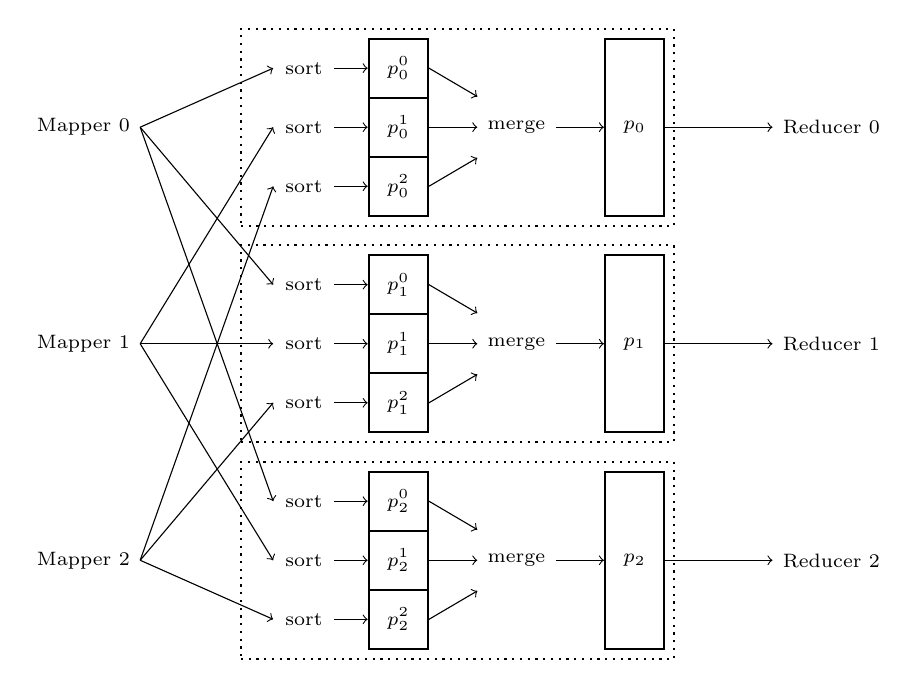
\begin{tikzpicture}[every node/.style={minimum height={0.75cm},minimum width={0.75cm},thick}]
      \node (Map2) at (0,1.25) {Mapper 2};
      \node (Map1) at (0,4) {Mapper 1};
      \node (Map0) at (0,6.75) {Mapper 0};

      \node[draw] (P20) at (4,2) { $p_2^0$ };
      \node[draw] (P21) at (4,1.25) { $p_2^1$ };
      \node[draw] (P22) at (4,0.5) { $p_2^2$ };
      \node (M2) at (5.5,1.25) {merge};
      \node (S20) at (2.8,2) {sort};
      \node (S21) at (2.8,1.25) {sort};
      \node (S22) at (2.8,0.5) {sort};
      \node[draw,minimum height={2.25cm}] (P2) at (7, 1.25) { $p_2$ };
      \node[draw,dotted,minimum height={2.5cm},minimum width={5.5cm}] at (4.75,1.25) {};

      \node[draw] (P10) at (4,4.75) { $p_1^0$ };
      \node[draw] (P11) at (4,4) { $p_1^1$ };
      \node[draw] (P12) at (4,3.25) { $p_1^2$ };
      \node (M1) at (5.5,4) {merge};
      \node (S10) at (2.8,4.75) {sort};
      \node (S11) at (2.8,4) {sort};
      \node (S12) at (2.8,3.25) {sort};
      \node[draw,minimum height={2.25cm}] (P1) at (7, 4) { $p_1$ };
      \node[draw,dotted,minimum height={2.5cm},minimum width={5.5cm}] at (4.75,4) {};

      \node[draw] (P00) at (4,7.5) { $p_0^0$ };
      \node[draw] (P01) at (4,6.75) { $p_0^1$ };
      \node[draw] (P02) at (4,6) { $p_0^2$ };
      \node (M0) at (5.5,6.75) {merge};
      \node (S00) at (2.8,7.5) {sort};
      \node (S01) at (2.8,6.75) {sort};
      \node (S02) at (2.8,6) {sort};
      \node[draw,minimum height={2.25cm}] (P0) at (7, 6.75) { $p_0$ };
      \node[draw,dotted,minimum height={2.5cm},minimum width={5.5cm}] at (4.75,6.75) {};

      \node (R2) at (9.5,1.25) {Reducer 2};
      \node (R1) at (9.5,4) {Reducer 1};
      \node (R0) at (9.5,6.75) {Reducer 0};

      \path [->](Map0.east) edge node {} (S00.west);
      \path [->](Map0.east) edge node {} (S10.west);
      \path [->](Map0.east) edge node {} (S20.west);
      \path [->](Map1.east) edge node {} (S01.west);
      \path [->](Map1.east) edge node {} (S11.west);
      \path [->](Map1.east) edge node {} (S21.west);
      \path [->](Map2.east) edge node {} (S02.west);
      \path [->](Map2.east) edge node {} (S12.west);
      \path [->](Map2.east) edge node {} (S22.west);

      \path [->](S00.east) edge node {} (P00.west);
      \path [->](S10.east) edge node {} (P10.west);
      \path [->](S20.east) edge node {} (P20.west);
      \path [->](S01.east) edge node {} (P01.west);
      \path [->](S11.east) edge node {} (P11.west);
      \path [->](S21.east) edge node {} (P21.west);
      \path [->](S02.east) edge node {} (P02.west);
      \path [->](S12.east) edge node {} (P12.west);
      \path [->](S22.east) edge node {} (P22.west);

      \path [->](P00.east) edge node {} (M0.north west);
      \path [->](P01.east) edge node {} (M0.west);
      \path [->](P02.east) edge node {} (M0.south west);
      \path [->](P10.east) edge node {} (M1.north west);
      \path [->](P11.east) edge node {} (M1.west);
      \path [->](P12.east) edge node {} (M1.south west);
      \path [->](P20.east) edge node {} (M2.north west);
      \path [->](P21.east) edge node {} (M2.west);
      \path [->](P22.east) edge node {} (M2.south west);

      \path [->](M0.east) edge node {} (P0.west);
      \path [->](M1.east) edge node {} (P1.west);
      \path [->](M2.east) edge node {} (P2.west);

      \path [->](P0.east) edge node {} (R0.west);
      \path [->](P1.east) edge node {} (R1.west);
      \path [->](P2.east) edge node {} (R2.west);
  \end{tikzpicture}
  \caption{Classical MapReduce programming model.}
  \label{fig:mapreduce}
\end{figure*}


% ############################################################################
\section{Literature Review} \label{sec:litrev}
% ############################################################################

The MapReduce programming model was initially introduced by Google in 2004 \cite{GoogleMapReduce} and later popularized by Yahoo! through the Apache open-source project Hadoop MapReduce \cite{Hadoop}.
Hadoop MapReduce provides a MapReduce runtime for networked commodity hardware and its popularity has resulted in the development of runtimes for alternative environments like GPU’s \cite{Mars}, FGPA's \cite{Melia}, Coprocessors \cite{MrPhi} and shared-memory systems \cite{Phoenix} \cite{Phoenix++} \cite{CilkMR} \cite{Metis} \cite{Ostrich}.

\subsection{Programming Model}

In the classical MapReduce programming model \cite{GoogleMapReduce}, illustrated
in Figure \ref{fig:mapreduce}, programmers only need to supply mapper and
reducer programs together with the source of the input and the destination of
the output, everything else is handled by the runtime. For most MapReduce
runtimes this means executing parallel workers running multiple instances of the
mapper and reducer programs, reading and distribution of the input, collection
and writing of the output and shuffling and sorting intermediate data. A
classical MapReduce job starts by splitting the input and running a mapper for
each split. Each mapper will consume the records in the split and output
key-value pairs which are collected by the runtime and partitioned into sorted
buckets. Key-value pairs with the same key end up in the same bucket no matter
which mapper produced the pair. Once all mappers are done a reducer is started
for each bucket and all key-value pairs in the bucket are processed in order.
This means that all key-value pairs with the same key will all be processed by
the same reducer. Finally, the output of the reducers becomes the output of the
job.

There is a lot of room for implementation specific deviations and optimizations
in this description but on a high level all MapReduce runtimes operates by this
model \cite{GoogleMapReduce} \cite{Hadoop} \cite{Phoenix} \cite{Phoenix++}
\cite{CilkMR} \cite{Metis} \cite{Ostrich}. The success of the MapReduce model
comes from the ease of writing sequential mapper and reducer programs that are
able to accomplish advanced data transformation tasks in parallel when executed
through a MapReduce runtime \cite{GoogleMapReduce}.

\subsection{Language support}

MapReduce runtimes with multi-language or language-agnostic support is not
something that has been greatly explored by the MapReduce community. In general
MapReduce runtimes are single language: Googles proprietary MapReduce is
described as a C++ runtime \cite{GoogleMapReduce}, Hadoop MapReduce provides a
runtime for Java \cite{Hadoop} and shared-memory runtimes like Phoenix
\cite{Phoenix}, Phoenix++ \cite{Phoenix++}, Metis \cite{Metis}, Ostrich
\cite{Ostrich} and CilkMR \cite{CilkMR} provide runtimes for C or C++.

In fact, the only available language-agnostic MapReduce runtime seems to be
Hadoop Streaming. Hadoop Streaming is built upon Hadoop MapReduce and achieves
language-agnostic support by replacing the mappers and reducers with externally
run processes that communicates with the MapReduce runtime over the standard
streams \cite{HadoopStreaming}. Unfortunately the MapReduce runtime that power
Hadoop Streaming is still the Java optimized Hadoop MapReduce runtime and the
resulting performance of Hadoop Streaming is very bad \cite{HadoopStreamingPerf}
\cite{Pydoop} \cite{Perldoop}. ShmStreaming is an attempt to increase the
performance of Hadoop Streaming by communicating over shared memory instead of
the standard streams \cite{ShmStreaming}. The performance of Hadoop Streaming +
ShmStreaming is superior to Hadoop Streaming but communication over shared
memory is not as straightforward to implement compared to communication over
standard streams. In addition, ShmStreaming still suffers from the fact that
Hadoop MapReduce is not optimized for interacting with mappers and reducers that
are run as external processes.

The Hadoop community has also developed Hadoop Pipes which outperforms Hadoop
Streaming but only offers support for C++ \cite{HadoopPipes}. Language support
for the python programming language without using Hadoop Streaming is available
through the Pydoop project. Pydoop integrates with Hadoop MapReduce by wrapping
Hadoop Pipes and offers superior performance versus running python mapper and
reducers through Hadoop Streaming \cite{Pydoop}. An alternative approach to
adding specific language support to Hadoop MapReduce was undertaken in the
Perldoop project \cite{Perldoop}. Perldoop provides a perl-to-java transpiler
specifically built to convert Perl Hadoop MapReduce jobs to Java Hadoop
MapReduce jobs. Perldoop can achieve very good performance since it is
effectively running regular Java Hadoop MapReduce however there are a lot of
limitations since only a subset of very specifically formatted Perl is
supported.

Finally, there seems to be no MapReduce runtime that is built explicitly for
multi-language or truly language-agnostic MapReduce.

\begin{figure}[h]
  \centering
  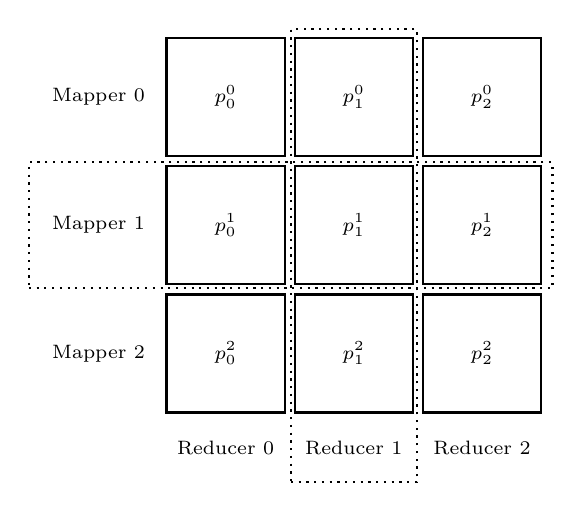
\begin{tikzpicture}[every node/.style={minimum height={1.5cm},minimum width={1.5cm},thick}]
    \matrix[row sep=1mm, column sep=1mm] (m)
    {
      \node { Mapper 0 }; & \node[draw] { $p_0^0$ }; & \node[draw] (c1) { $p_1^0$ }; & \node[draw] { $p_2^0$}; \\
      \node (r1) { Mapper 1 }; & \node[draw] { $p_0^1$ }; & \node[draw] { $p_1^1$ }; & \node[draw] { $p_2^1$ }; \\
      \node { Mapper 2 }; & \node[draw] (node0) { $p_0^2$}; & \node[draw] (node1) { $p_1^2$ }; & \node[draw] (node2) { $p_2^2$ }; \\
    };

    \node[below=1.75cm of node0.north,minimum height=0cm] {Reducer 0};
    \node[below=1.75cm of node1.north,minimum height=0cm] {Reducer 1};
    \node[below=1.75cm of node2.north,minimum height=0cm] {Reducer 2};

    \node[below=-1.1mm of c1.north,draw,dotted,minimum height=5.75cm,minimum width=1.6cm] {};
    \node[below right=-0.5mm and -0.9cm of r1.north,draw,dotted,minimum height=1.6cm,minimum width=6.65cm] {};
  \end{tikzpicture}
  \caption{Memory layout in shared-memory MapReduce runtimes.}
  \label{fig:memorylayout}
\end{figure}


\subsection{Shared-memory}

Shared-memory systems are becoming increasingly capable and cost effective for
data processing. At the time of writing it is possible to get a on demand system
with 128 cores and 3.9TB of memory \cite{AWS}. Based on
recent releases from popular cloud providers the trend of access to high
core-count systems is likely to continue and cost per core will likely keep
decreasing \cite{AWS} \cite{GoogleCloud}.

MapReduce on shared-memory systems was first explored by the Phoenix
\cite{Phoenix} project. Besides being first to explore MapReduce on
shared-memory systems the Phoenix project also contributed the matrix
memory-layout illustrated in Figure \ref{fig:memorylayout}. This memory layout
is used in some form by all shared-memory runtimes \cite{Phoenix}
\cite{Phoenix++} \cite{CilkMR} \cite{Metis} \cite{Ostrich} and enables workers
to communicate extremely efficiently with the runtime while avoiding contention.
The columns in the matrix represent buckets and each entry in the matrix is a
buffer responsible for storing the intermediate data produced by a mapper.
During the mapper stage each mapper is given access to a row in the matrix and
during the reducer stage each reducer is given access to a column in the matrix.
This methodology ensures that no communication is required across workers during
execution which in turns maximizes throughput.

The Phoenix runtime has gone through multiple iterations and Phoenix 2.0 was the
result of performance issues when Phoenix was run on larger shared-memory
systems processing larger data sets \cite{Phoenix2}. In particular the
intermediate data buffers that are used to store keys from the key-value pairs
produced by the mappers are implemented as sorted arrays in Phoenix. This lead
to performance issues since the arrays needed to reallocate whenever they ran
out of space and whenever a new key was added all keys coming after the new key
had to be shifted. Phoenix 2.0 solved this issue by significantly increasing the
number of sorted key arrays so that on average only one key resides in each
array \cite{Phoenix2}.

Further work on the Phoenix project has lead to the determination that the
intermediate sorted arrays were limiting the potential performance of the
runtime. This resulted in the reimplementation of Phoenix in C++ and the start
of the Phoenix++ project \cite{Phoenix++}. Phoenix++ is the poster child of
shared-memory MapReduce runtimes optimized for speed and extends the MapReduce
API to include containers and combiner objects. Containers exposes the internals
of the shuffle stage to the programmer and makes it possible to select or tune
the data structure used for shuffling \cite{Phoenix++}. Combiner objects exposes
the internals of the intermediate data buffers and makes it possible to select
the data structure used for intermediate data buffering \cite{Phoenix++}. While
the introduction of containers and combiner objects in Phoenix++ does allow for
better performance it has been argued that they break the MapReduce abstraction
and programmers now need to be intimately familiar with the Phoenix++ internals
to pick the correct containers and combiner objects \cite{CilkMR}.

An alternative approach to dealing with the perceived shortcomings of the
Phoenix project is the Metis project. Instead of increasing the configurability
of the runtime Metis introduces a compromise intermediate data buffer
\cite{Metis}. Using a more advanced buffer Metis is able to achieve significant
performance increase over Phoenix on data processing problems involving very
little mapper/reducer computation on datasets with few keys but many duplicates.
Metis does not offer any performance increase over Phoenix on data processing
jobs involving a significant amount of mapper/reducer computation or on datasets
with few duplicate keys \cite{Metis}.

An extension of the Phoenix model is Tiled-MapReduce and its prototype
implementation Ostrich. Ostrich extends the model introduced by Phoenix by using
the tiling strategy commonly used in the compiler community. Ostrich and
Tiled-MapReduce in general splits the input into subsets and runs smaller jobs on each
subset. Each smaller job runs mappers that produces a intermediate data buffer
like Phoenix but then reduces the partial intermediate data buffer using a
combiner into a secondary intermediate data buffer. Once all smaller jobs have
run the secondary intermediate data buffers are reduced by the reducers. Since
the combiner reduces the amount of intermediate data this approach increases the
performance of the runtime and allows for processing of more data. In addition
the primary intermediate data buffer that is filled by the mappers can be reused
between the smaller jobs. This means that Ostrich is able to avoid a lot of
memory allocation calls compared to Phoenix and other shared-memory runtimes
\cite{Ostrich}.

\begin{figure*}[h]
\begin{lstlisting}
Usage: xrt [--help] [--version] <options>

Resource options:
  --workers <num>  set the number of workers to <n> (default: 4)
  --memory <mem>   set the amount of allocated memory (default: 256m)
  --tempdir <dir>  set the temporary directory (default: system temporary directory)

Job options:
  --input <file|dir>  input file or directory
  --mapper <cmd>      mapper command (required)
  --reducer <cmd>     reducer command
  --output <dir>      output directory
\end{lstlisting}
\caption{XRT usage options}
\label{fig:xrt}
\end{figure*}

The CilkMR project is one of the newest MapReduce runtimes for shared-memory
systems and addresses the key-value pair serialization/deserialization overhead
of all the previously discussed runtimes \cite{CilkMR}. Instead of operating on
key-value pairs CilkMR operates over typed data containers which means that the
mappers can pass arbitrary data structures to the reducers. CilkMR is also
inspired by Phoenix++ in that it allows the programmers to control intermediate
data structures and tune the runtime. The performance of CilkMR is really good
on computationally heavy tasks since mappers and reducers can operate on complex
data structures. However, Phoenix++ performs better than CilkMR on classical
data processing jobs like word-count and string-search \cite{CilkMR} \cite{GoogleMapReduce}.

A completely different idea for bringing MapReduce to shared-memory systems is
the Hone project. Hone attempts to take advantage of the familiarity of Hadoop
MapReduce by providing a Hadoop MapReduce compatible Java API
\cite{ScalingDown}. The goal is to create a runtime that allow you to run the
exact same Java code that was written for Hadoop MapReduce. In benchmarks Hone
beats Phoenix however Phoenix++ beats Phoenix by a much wider margin and thus it
seems like Phoenix++ is likely much faster then Hone.

A last note about recent development in shared-memory MapReduce runtimes is the
usage of disk based data structures. In Hadoop MapReduce almost all intermediate
data will reside on disk at some point but in all the above mentioned
shared-memory runtimes there is never a mention of disk backing. There has been
some exploration in extending Metis to include the capacity of spilling
intermediate data to disk if the input is too large \cite{DiskOptimization}.
However, this optimization was never contributed back to the Metis project.

% ############################################################################
\section{XRT 0.1.0} \label{sec:xrt}
% ############################################################################

XRT 0.1.0 is the first release of the XRT MapReduce runtime for shared-memory systems.
The objective of XRT is to offer a simple, high-performance, resource-aware and language-agnostic MapReduce runtime.
Internally XRT is based on ideas developed in shared-memory MapReduce systems like Phoenix \cite{Phoenix} combined with language-agnostic concepts from Hadoop Streaming \cite{HadoopStreaming}.
In addition, it explores novel topics in the shared-memory MapReduce space like resource awareness and the ability to use secondary storage for datasets that do not fit in memory.
XRT is being implemented in the Go language and Figure \ref{fig:xrt} shows the usage options of XRT.

To keep usage simple and enable truly language-agnostic support XRT is built to operate on newline-delimited data.
Widely used formats like csv, tsv and newline delimited json can all be used.
On a high level XRT follows the classical MapReduce model illustrated in Figure \ref{fig:mapreduce} and programming MapReduce jobs involves writting mapper and reducer programs.

XRT mapper programs read newline-delimited records from stdin and writes newline-delimited worker-id/record pairs to stdout.
The XRT runtime shuffles the records by the associated worker-id and then sorts the records before passing them to the reducer program.

XRT reducer programs read sorted newline-delimited records from stdin and writes newline-delimited records to stdout which in turn becomes the output of the MapReduce job.

% ----------------------------------------------------------------------------
\subsection{Examples} \label{sec:examples}
% ----------------------------------------------------------------------------

Here are a few common MapReduce tasks to illustrate usage of the XRT MapReduce runtime.

\bigskip
\noindent
\textbf{string-search:} The mapper program reads records from stdin and only writes records to stdout that matches the search pattern. No reducer program is needed.

\bigskip
\noindent
\textbf{word-count:} The mapper program reads words from stdin, assigns a worker-id to each word to ensure that all words that are the same end up on the same reducer.
The reducer program reads a word from stdin and keeps reading as long as new words is the same as the first word while keeping a count of how many words have been read.
When a new word is read from stdin that does not match the first word the reducer writes the current word and the associated count to stdout and then restarts the process with the new word.

\bigskip
\noindent
\textbf{sort:} The mapper program reads records from stdin and assigns a worker-id to the record such that records ending up on reducer\textsubscript{i} are all smaller then records ending up on reducer\textsubscript{i+1}.
The reducer program reads records from stdin in sorted order and simply pass them to stdout as all sorting and partitioning needed has already been completed by the runtime.

% ############################################################################
\section{Implementation} \label{sec:impl}
% ############################################################################

The flow of records through a XRT MapReduce job is split into 9 distinct subroutines out of which 4 are visible to the user (input, mapper, reducer, output) and 5 are internal to the runtime (shuffle, buffers, spilling, merging).
In this section the technical details of each subroutine is described in order of execution for a typical XRT job.

\bigskip
\noindent
\textbf{input:} Input can be a single or multiple files containing newline-delimited records.
The XRT runtime enumerates the input files and assigns 64mb chunks from the input to the mapper programs while ensuring that each chunk starts and end at newline boundaries.

\bigskip
\noindent
\textbf{mapper:} Mapper programs read newline-delimited records from stdin, processes the record, assigns a worker-id to each record and writes the worker-id/processed-record pair to stdout.
The worker-id will be used by the runtime to shuffle the record to the appropriate reducer program.
The number of mapper programs that will be started by the XRT runtime is determined by the number of workers configured.

\bigskip
\noindent
\textbf{shuffle:} Shuffle receives the worker-id/processed-record pairs from the mapper programs and shuffles them to the appropriate buffer based on worker-id.

\bigskip
\noindent
\textbf{buffers:} Buffers are implemented using the matrix memory model illustrated in Figure \ref{fig:memorylayout} which means that for each mapper program there is a associated list of buffers, one for each reducer program.
Records are directed to a buffer by the shuffle which can be done lock-free due to the matrix based memory layout.
The current implementation of XRT uses a simple byte buffer where pointers to records are prepended and the records themselves are appended.

\bigskip
\noindent
\textbf{spilling:} Spilling occurs when a buffer becomes full, meaning the free space between the prepended record pointers and the appended records is too small to hold additional pointers and records.
During spilling the full buffer is sorted, written out to disk and then cleared.

\bigskip
\noindent
\textbf{sort:} Sort starts once all mapper programs have terminated.
It first sorts the in memory records by only moving the record pointers, reducing the number of bytes that need to be moved around while also making it possible to sort in place.
If any buffers spilled then sort uses a external heap-based n-way merge to create a single sorted file for each buffer.

\bigskip
\noindent
\textbf{merging:} Merging grabs all in-memory buffers and all on-disk spill files associated with a reducer and using a heap-based n-way merge creates a single sorted stream of records.

\bigskip
\noindent
\textbf{reducer:} Reducer programs read the sorted stream of records from the merging phase which are delivered to the reducer program over stdin.
The reducer program processes the records and writes them to stdout.
The number of reducer programs that will be started by the XRT runtime is determined by the number of workers configured.

\bigskip
\noindent
\textbf{output:} The records written to stdout by the reducer programs are written to a temporary location on disk.
Once all reducer programs have finished successfully XRT commits the data by moving the temporary data to the target output directory.

% ############################################################################
\section{Performance} \label{sec:perf}
% ############################################################################

In this section we present the results of running common MapReduce tasks using XRT 0.1.0 on a large shared-memory system.

\subsection{System setup}

The shared-memory system had 32 cores, 224GB of memory, one 500GB SSD disk and was running a default Ubuntu 16.04 installation.
XRT was compiled using Go 1.9.1 and the mapper and reducer programs were implemented in Python and executed by Python 2.7.11.
Execution times were collected using the linux time command.

\subsection{Dataset}

A artificial 50GB dataset was generated and contained 500 million 100-byte records.
The dataset was split into 50, 1GB files each containing 10 million 100-byte records.
The records were split into a 5-byte key followed by a tab-character followed by a 93-byte payload followed by a newline-character.
Every byte in every record was randomly picked from the sequence of lowercase characters in the range a-z.

\subsection{Benchmarks}

We ran the 3 examples from Section \ref{sec:examples} as our benchmarks with the following implementation details.

\bigskip
\noindent
\textbf{string-search:} The mapper program reads records from stdin and only writes records to stdout if the first 5-character of the 93-byte payload are all the character 'a'.

\bigskip
\noindent
\textbf{word-count:} The mapper program reads records from stdin and sets the worker-id for each record using a hash of the 5-byte key modulo the number of workers.
The mapper program only emits the worker-id/key pair as we are only interested in a count by key.
The reducer program counts the number of times a key is observed and emits the current key and current count to stdout when a new key is read from stdin.

\bigskip
\noindent
\textbf{sort:} The mapper program reads records from stdin and assigns a worker-id to each record ensuring that records assigned to worker\textsubscript{i} are guaranteed to be smaller then records assigned to worker\textsubscript{i+1}.
The reducer program reads records from stdin and simply write them to stdout directly as they are already in sorted order.

\subsection{Results}

\subsubsection{Baseline}

For the first performance evaluation each of the benchmarks were implemented as optimal and sequential non-MapReduce programs.
These baseline implementations where then compared with the performance of the XRT MapReduce implementations.
When number of XRT workers was set to 1 the baseline implementations where on average 20\% faster due to the overhead incurred by the XRT runtime.
When the number of workers was increased to 2 XRT was able to completely outperform the optimal sequential implementations.

\begin{figure}[h]
  \centering
  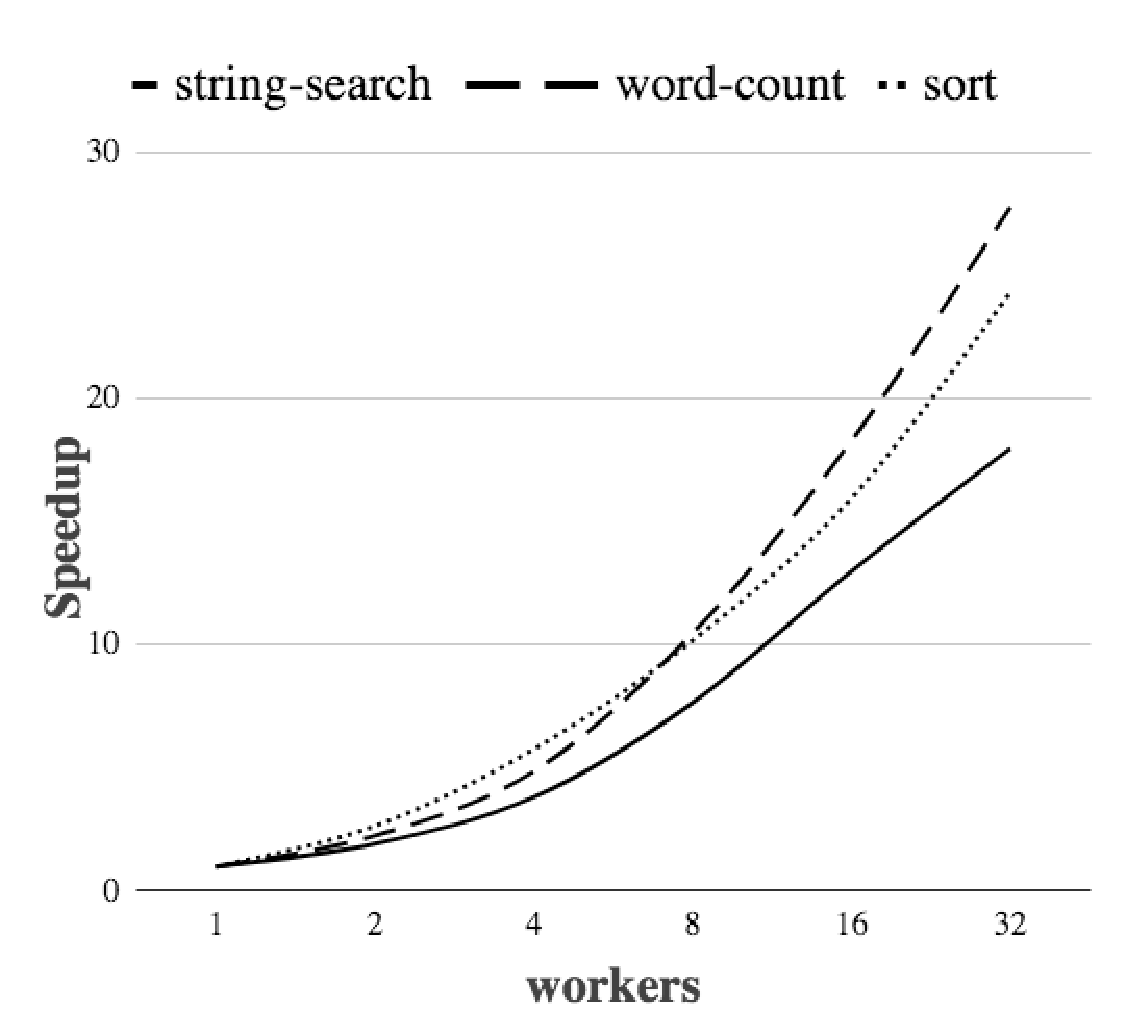
\includegraphics[width=8cm]{graph.eps}
  \caption{Speedup of XRT as worker counts are increased}
  \label{fig:perf}
\end{figure}

\subsubsection{Speedup}

Figure \ref{fig:perf} shows the speedup of string-search, word-count and sort as the number of XRT workers is increased.
The results show that we are approximately doubling the speedup as we double the core count which is precisely the kind of speedup that we're aiming to achieve.
The job with the lowest speedup is string-search which also happens to be the least computationally heavy job and thus is likely bottlenecked by the fact that our benchmarking system only has a single SSD.
We also see that as we approach 32 workers we have a bit of a reduction in speedup across all benchmarks.
Again this is likely due to the single SSD becoming a bottleneck.

% ############################################################################
\section{Conclusion} \label{sec:concl}
% ############################################################################

This paper introduced XRT 0.1.0, a novel language-agnostic MapReduce runtime for shared-memory systems.
The implementation details of XRT were explored and through our benchmarks we have shown that XRT enables high-performance data processing with a good speedup profile as core-counts increase.

Furthermore, we have shown that XRT addresses the perceived shortcomings and lacks in the shared-memory MapReduce community.
XRT is language-agnostic and memory first but can process datasets that do not fit in memory by having first class support for spilling to disk.
In addition, we believe XRT to be heading towards a industry-ready state with easy development, deployment and management as well as a robust implementation.

We intend to continue optimizing the various internal components of XRT and run further benchmarks on even larger shared-memory systems.
In particular, we are interested in running benchmarks on shared-memory systems with multiple RAID mounted SSD's to address the slight slowdowns we observed in our performance evaluation.
We are also intersted in exploring performance on skewed datasets as well as datasets which force XRT to spill to disk.

Overall, we believe that we have shown that language-agnostic shared-memory MapReduce is possible and extremely attractive following the advent of high core-count shared-memory systems.

% ############################################################################
% Bibliography
% ############################################################################
\bibliographystyle{plain}
\bibliography{bibliography}     %loads bibliography.bib

% ============================================================================

\end{document}

